\documentclass{physics_article_B}

\mytitle{Fitting Radial Velocity Curves Using N-Body Problem Modelling}
\studentid{14306575}
\date{\today}

\addbibresource{references.bib}

\usepackage{lipsum}

\setlength{\columnsep}{0.7cm}

\begin{document}
\maketitle

\begin{abstract}
This report discusses the use of a python program to solve the N-body problem and then use the trajectories to fit empirical radial velocity data to the model. The N-body problem is not generally solvable analytically therefore the fourth-order Runge-Kutta method is used to solve coupled equations in three dimensions when given initial conditions. Tooling was also developed to aid the use of the program. Results are cached so the same initial conditions never need to be determined more than once. Plotting including real-time animations, energy and angular momentum are also supplied in the repository. A good fit for a simple exoplanetary system is found for the radial velocity data.
\end{abstract}

\section{Introduction}

When Newton's Principia Mathematica was published, it allowed the motions of the planets around the Sun to be understood by applying Newton's Laws. Each planet and the Sun could be approximated as a two-body system. Newton's Laws were then used to solve the two-body problem and this allowed Kepler's three empirical laws to be confirmed. This report tackles the more complex N-body problem using numerical methods.

\subsection{Newton's Laws}
This subsection outlines the prerequisites to solve the two-body problem. Alongside Newton's three laws of motion, he presented his Universal Law of Gravitation. Mathematically, for two-point masses labelled $i$ and $j$ the gravitational force exerted on the mass $m_i$ due to the mass $m_j$ is

\begin{equation}
\vec{F}_{j\rightarrow i} = -\frac{Gm_im_j}{r_{ij}^2}\hat{r}_{ij}
\label{eq:gravitationforce}
\end{equation}

where $G$ is the universal gravitational constant, $r_{ij}$ is the distance between the two masses and the unit vector $\hat{r}_{ij}$ is the direction from the $i^{th}$ mass to the $j^{th}$ mass \cite{hartle_gravity_2003}.

This prescription can further be used to describe the forces and thus motions of planets. Newton's Spherical Shell Theorem states that spherically symmetric bodies can be considered as point masses. Concretely, all the mass of a planet can be treated as if it were at the centre of the planet. Therefore, as the planets can be approximated as spheres and so \cref{eq:gravitationforce} applies.

\subsection{The N-Body Problem}
After the two-body problem was solved it was the natural progression to tackle the three-body problem. Newton attempted to solve the system consisting of the Sun, Moon and Earth analytically but failed \cite{hartle_gravity_2003}. It's impossible to solve, in general, the N-body problem analytically for $n\ge 3$. This report tackles computed solutions to this problem making use of numerical solvers.

To define the problem in mathematics let the $N$ bodies have masses $m_i$ where the bodies have been given the integer label $i$; positions $\vec{x}^{(i)} = (x^{(i)},y^{(i)}, z^{(i)})$ which is in three dimensions; and velocities $\dot{\vec{x}}^{(i)} = (\dot{x}^{(i)},\dot{y}^{(i)},\dot{z}^{(i)})$ which are independent of the positions. Here the dots represent time derivatives.

The net force on mass $m_i$ is the vector sum of all the forces exerted by the other masses. Using label $j$ defined so $j\neq i$ this can be written as

\begin{equation}
\vec{F}_i = -G\sum_{\substack{j=1\\j\neq i}}^N\frac{m_im_j(\vec{x}^{(i)} - \vec{x}^{(j)})}{|\vec{x}^{(i)} - \vec{x}^{(j)}|^3}
\label{eq:ithforce}
\end{equation}

where the unit vector has been expanded. Using Newton's second law for constant mass the acceleration of the mass $m_i$ can be written as $\vec{F}_i = m_i\ddot{\vec{x}}^{(i)}$. Therefore, cancelling mass $m_i$ \cref{eq:ithforce} can be written as

\begin{equation}
 \ddot{\vec{x}}^{(i)} = -G\sum_{\substack{j=1\\j\neq i}}^N\frac{m_j(\vec{x}^{(i)} - \vec{x}^{(j)})}{|\vec{x}^{(i)} - \vec{x}^{(j)}|^3}.
 \label{eq:vectormotion}
\end{equation}

This is a second-order ordinary differential equation. Which can be solved using various methods once written as two coupled first-order equations:

\begin{equation}
 \label{eq:vectorcoupled}
\left\{
 \begin{array}{@{}ll@{}}
 \dot{\vec{v}}^{(i)} = -G\sum_{j=1, j\neq i}^N\frac{m_j(\vec{x}^{(i)} - \vec{x}^{(j)})}{|\vec{x}^{(i)} - \vec{x}^{(j)}|^3}\\
 \dot{\vec{x}} = \vec{v}\\
 \end{array}\right.
\end{equation}

where the new variable $\vec{v} = (v_x, v_y, v_z)$ has been introduced.

Gravitational systems such as the Solar System should have conserved quantities as they are closed systems. These are a good metric to check whether a solver calculates the trajectories correctly. Firstly the total energy $E$ of a system should be conserved. For systems where the only interaction is gravitation, $E = U + T$, where $U$ is the gravitational potential energy and $T$ is the kinetic energy. For an N-body system, these can be defined as

\begin{equation}
 U = -\sum_{i=1}^N\sum_{\substack{j=1,\\ j > i}}^N\frac{Gm_im_j}{|\vec{x}^{(i)} - \vec{x}^{(j)}|}
 \label{eq:gravpotential}
\end{equation}
\begin{equation}
 T = \frac{1}{2}\sum_{i=1}^Nm_i|\dot{\vec{x}}^{(i)}|^2
 \label{eq:kinetic}
\end{equation}

where the energy terms are not double-counted in the second summation for the potential energy. Another quantity that should be conserved is the angular momentum $\vec{L}$. This is defined with the vector sum

\begin{equation}
 \vec{L} = \sum_{i=1}^N\vec{x}^{(i)}\times(m_i\dot{\vec{x}}^{(i)})
 \label{eq:angmom}
\end{equation}

which is in terms of vector products between the positions and linear momenta vectors.

\section{Model}

There are many numerical solvers for ordinary differential equations. Systems of the form $\dot{x} = f(x, t)$ can be solved using the explicit Runge-Kutta method of order 5(4) \cite{dormand_family_1980} when given the initial conditions $x(0) = x_0$. This report employs an implementation of this algorithm.

This method is an improvement of the famous Euler's method. The algorithm starts an iterative method with the initial conditions. That is the initial value $(0, x_0)$ corresponds to $n=0$. Through the use of a Taylor expansion of $f(x, t)$, the value of the solution at a position $h$ is approximated to fourth-order by taking four steps along the way. In the fourth-order version of the Runge-Kutta method, the iterative formula is \cite{press_numerical_1992}

\begin{equation}
 x_{n+1} = x_n + \frac{k_1}{6} + \frac{k_2}{3} + \frac{k_3}{3} + \frac{k_4}{6} + \mathcal{O}(h^5)
 \label{eq:rungekutta54}
\end{equation}

where the $k$ terms are defined as

\begin{equation}
 \begin{aligned}
 k_1 &= hf(x_n, t_n) \\
 k_2 &= hf(x_n + k_1/2, t_n + h/2) \\
 k_3 &= hf(x_n + k_2/2, t_n + h/2) \\
 k_4 &= hf(x_n + k_3, t_n + h) \\
 \end{aligned}
\end{equation}

where $h$ is the chosen step-size. For the implementation, the higher-order terms, denoted by $\mathcal{O}(h^5)$, are ignored. This method is an accurate approximation to $\dot{x} = f(x, t)$ to fourth-order in the total error. The solver used in this project makes use of an adaptive step size. This means the algorithm chooses $h$ on each iteration to ensure it is accurate when $f(x, t)$ varies greatly but is not too slow when the function does not vary significantly \cite{press_numerical_1992}. For the scenario presented here, this algorithm has an approximate worst-case time complexity of $O(mN^2)$ where $m$ is the number of time steps being used and $N$ is the number of bodies. This means for a small number of bodies it is approximately linear in time but for a large number of bodies, it becomes quadratic in time. This is fine for the applications in this report as the number of bodies is small but it will become problematic for modelling systems with more bodies.

The RK4(5) algorithm requires first-order differential equations. \Cref{eq:vectorcoupled} is rewritten as a set of $6N$ coupled first-order differential equations below --- one for each position and velocity component:

\begin{equation}
 \left\{
 \begin{array}{@{}ll@{}}
 \dot{v_x}^{(1)} &= -G\sum_{j = 1,j\neq 1}^N\frac{m_j(x^{(1)} - x^{(j)})}{|\vec{x}^{(1)} - \vec{x}^{(j)}|^3}\\
 \dot{v_y}^{(1)} &= -G\sum_{j = 1,j\neq 1}^N\frac{m_j(y^{(1)} - y^{(j)})}{|\vec{x}^{(1)} - \vec{x}^{(j)}|^3}\\
 \dot{v_z}^{(1)} &= -G\sum_{j = 1,j\neq 1}^N\frac{m_j(z^{(1)} - z^{(j)})}{|\vec{x}^{(1)} - \vec{x}^{(j)}|^3}\\
 &\vdots\\
 \dot{v_x}^{(N)} &= -G\sum_{j = 1,j\neq N}^N\frac{m_j(x^{(N)} - x^{(j)})}{|\vec{x}^{(N)} - \vec{x}^{(j)}|^3}\\
 \dot{v_y}^{(N)} &= -G\sum_{j = 1,j\neq N}^N\frac{m_j(y^{(N)} - y^{(j)})}{|\vec{x}^{(N)} - \vec{x}^{(j)}|^3}\\
 \dot{v_z}^{(N)} &= -G\sum_{j = 1,j\neq N}^N\frac{m_j(z^{(N)} - z^{(j)})}{|\vec{x}^{(N)} - \vec{x}^{(j)}|^3}\\
 \dot{x}^{(1)} &= v_x^{(1)}\\
 \dot{y}^{(1)} &= v_y^{(1)}\\
 \dot{z}^{(1)} &= v_z^{(1)}\\
 &\vdots\\
 \dot{x}^{(N)} &= v_x^{(N)}\\
 \dot{y}^{(N)} &= v_y^{(N)}\\
 \dot{z}^{(N)} &= v_z^{(N)}\\
 \end{array}\right.
 \label{eq:coupledeqns}
\end{equation}

This is done to solve the system with a single function call. The numerical values of the subjects of these equations are bundled into a vector. Likewise, the initial conditions are bundled the same way:

\begin{equation}
 \vec{X}(t) =
 \begin{pmatrix}
 v_x^{(1)}(t) \\ \vdots \\ v_x^{(N)}(t) \\ v_y^{(1)}(t) \\ \vdots \\ v_y^{(N)}(t) \\ v_z^{(1)}(t) \\ \vdots \\ v_z^{(N)}(t) \\ x^{(1)}(t) \\ \vdots \\ x^{(N)}(t) \\ y^{(1)}(t) \\ \vdots \\ y^{(N)}(t) \\ z^{(1)}(t) \\ \vdots \\ z^{(N)}(t)
 \end{pmatrix}
 \qquad\qquad
 \vec{X}(0) = \begin{pmatrix}
 v_x^{(1)}(0) \\ \vdots \\ v_x^{(N)}(0) \\ v_y^{(1)}(0) \\ \vdots \\ v_y^{(N)}(0) \\ v_z^{(1)}(0) \\ \vdots \\ v_z^{(N)}(0) \\ x^{(1)}(0) \\ \vdots \\ x^{(N)}(0) \\ y^{(1)}(0) \\ \vdots \\ y^{(N)}(0) \\ z^{(1)}(0) \\ \vdots \\ z^{(N)}(0)
 \end{pmatrix}
 .
 \label{eq:statevector}
\end{equation}

The initial conditions are passed to the solver algorithm along with the time-domain for the trajectories. To configure the accuracy of the solutions the maximum step size needs to be chosen so the trajectories do not diverge too quickly.

The solver requires a function that calculates and returns the derivatives from \cref{eq:coupledeqns}. The function is provided with the vector $\vec{X}$ at a time $t$. The constants of the problem are provided through partial function application where a the masses and the value of $G$ are bound before the solver starts. The algorithm for calculating the derivatives is vectorised and is outlined now.

The vector is first divided back into individual position and speed components. These are each a 1D vector of length $N$. To calculate the separations, the difference between the vector and its transpose it calculated. This broadcasting operation is demonstrated in \cref{eq:broadcasting} for the $x$-component.

\begin{equation}
 \vec{x} - \vec{x}^T =
 \begin{pmatrix}
 x^{(1)} \\ x^{(2)} \\ \vdots \\ x^{(N)}
 \end{pmatrix}
 -
 \begin{pmatrix}
 x^{(1)} & x^{(2)} & \cdots & x^{(N)}
 \end{pmatrix}
 =
 \begin{pmatrix}
 0 & x^{(1)} - x^{(2)} & \cdots & x^{(1)} - x^{(N)} \\
 x^{(2)} - x^{(1)} & 0 & \cdots & x^{(2)} - x^{(N)} \\
 \vdots & \vdots & \ddots & \vdots \\
 x^{(N)} - x^{(1)} & x^{(N)} - x^{(2)} & \cdots & 0 \\
 \end{pmatrix}
 \label{eq:broadcasting}
\end{equation}

This is an antisymmetric matrix so the upper triangle is the opposite sign to the lower triangle. With a matrix for each spatial dimension, the cube of the separations can be determined as in \cref{eq:coupledeqns} by calculating the sum of the element-wise squares of the matrices then raising each element to a power of $3/2$. The values along the diagonal are then set to infinity as it would otherwise result in division by zero errors. The accelerations for each component due to each mass can then be calculated by dividing the individual separation matrices, element-wise, by the cubed separations. These matrices are of the same shape. This matrix is then multiplied by the mass vector, another broadcasting operation. The total acceleration of each mass is then the sum of each row of this new $N\times N$ matrix finally multiplied by $-G$.

The expected return value of this function is a vector similar to \cref{eq:statevector} which is referred to as the state. The speed values are unchanged like in \cref{eq:coupledeqns}.

\subsection{Units}
For physically meaningful solutions the units need to be chosen. Many unit choices exist however some will result in more numerical errors when quantities are typically large or small. This report makes use of two which are summarised in \cref{tab:unitsys}. These keep the magnitude of the systems studied around unity.

\begin{table}[H]
 \centering
 \caption{Unit systems used in this project. AU, $\mathrm{M_\odot}$, yr are astronomical units, solar masses and years respectively.}

 \setlength{\tabcolsep}{0.5em}
 \renewcommand{\arraystretch}{1.5}
 \begin{tabular}{|c|c|c|c|c|}
 \hline
 System & $G$ & $m_i$ & $\vec{x}^{(i)}$ & $\dot{\vec{x}}^{(i)}$ \\
 \hline
 Dimensionless & 1 & 1 & 1 & 1 \\
 Astronomical & $\simeq 40.2\ \mathrm{AU^3\ M_\odot^{-1}\ yr^{-2}}$ & $M_\odot$ & AU & $\mathrm{AU\ yr^{-1}}$ \\
 \hline
 \end{tabular}
 \label{tab:unitsys}
\end{table}

SI units could be used however they make the values tedious to enter and since most of the literature presents values in astronomical units it makes sense to continue with that convention.

\subsection{Tooling}

Several tools were developed to aid the use of this software. When a large time step, a large number of bodies or a long duration is used the runtime can take around ten seconds to a couple of minutes to execute. For this reason, an automatic caching system was developed. This system stores a representation of the initial values (a SHA256 hash) along with the calculated trajectories after being calculated for the first time. Therefore, if the same initial values are used again, the system does not need to be solved for a second time but instead the values can be loaded from storage. This is automatic so the user does not need to worry about storing the values or loading data.

The initial values are loaded from JSON files (Javascript Object Notation). This is a simple text file data structure that allows the initial values for many systems to be saved and then loaded and solved.

\section{Testing the Model}
To test the implementation, a few systems with known results are used to see if the produced trajectories are similar.

\subsection{Two Body Problem}
\label{ssec:twobody}
The simplest test is a two-body system where the bodies have equal mass. The initial conditions can be found in the \texttt{bodies/twobodies.json} file in the repository \cite{dudgeon_oliverdudgeon/nbody_2019}. The units of those initial values are given in the dimensionless unit scheme outlined in \cref{tab:unitsys}. The analytical solutions to this problem give elliptical solutions as shown in \cref{fig:twobodies}

\begin{figure}[h]
 \centering
 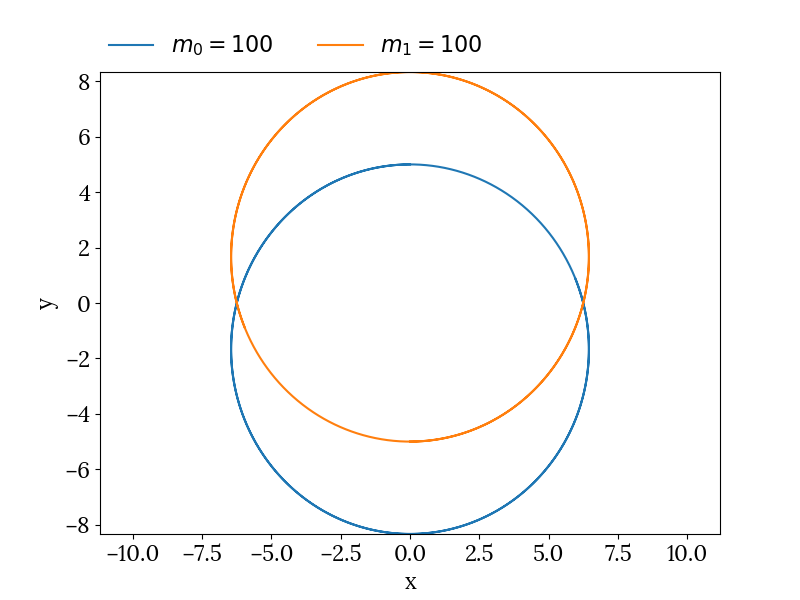
\includegraphics[width=0.8\linewidth]{twobodies.png}
 \caption{Trajectories of the two bodies. The orbits are circular each about the combined centre of mass. }
 \label{fig:twobodies}
\end{figure}

The relative change in the total energy from the initial value is calculated as: $E(t)/E(0) - 1$ using the energy definitions from \cref{eq:gravpotential} and \cref{eq:kinetic}. This shows it is conserved to the degree that it varies on the order of $10^{-8}$ around zero total energy. This is within the allowance from numerical errors from the solver.

Furthermore, following the same argument for angular momentum which was calculated using \cref{eq:angmom} also shows it is conserved. It only varies on the order of $10^{-9}$ around zero total angular momentum.

This test shows that the correct trajectories are produced with conserved energies and angular momenta.

\subsection{Figure of Eight}
This is a three-body problem with solutions proven to have the three bodies following a single figure of eight path with each body appearing to chase the others \cite{chenciner_remarkable_2000}. The initial conditions are given in \cref{tab:figure8init}.

\begin{table}[H]
 \centering
 \caption{Initial conditions for the figure of eight system. Values given in dimensionless units.}

 \setlength{\tabcolsep}{0.5em}
 \renewcommand{\arraystretch}{1.5}
 \begin{tabular}{|c|c|c|c|c|c|c|}
 \hline
 $m$ & $x_0$ & $y_0$ & $z_0$ & $v_{x0}$ & $v_{y0}$ & $v_{z0}$ \\
 \hline
 1 & 0.97000436 & -0.24308753 & 0 & 0.466203685 & 0.4323657 & 0 \\
 1 & -0.97000436 & 0.24308753 & 0 & 0.466203685 & 0.43236573 & 0 \\
 1 & 0 & 0 & 0 & -0.93240737 & -0.86473146 & 0 \\
 \hline
 \end{tabular}
 \label{tab:figure8init}
\end{table}

\begin{figure}[H]
 \centering
 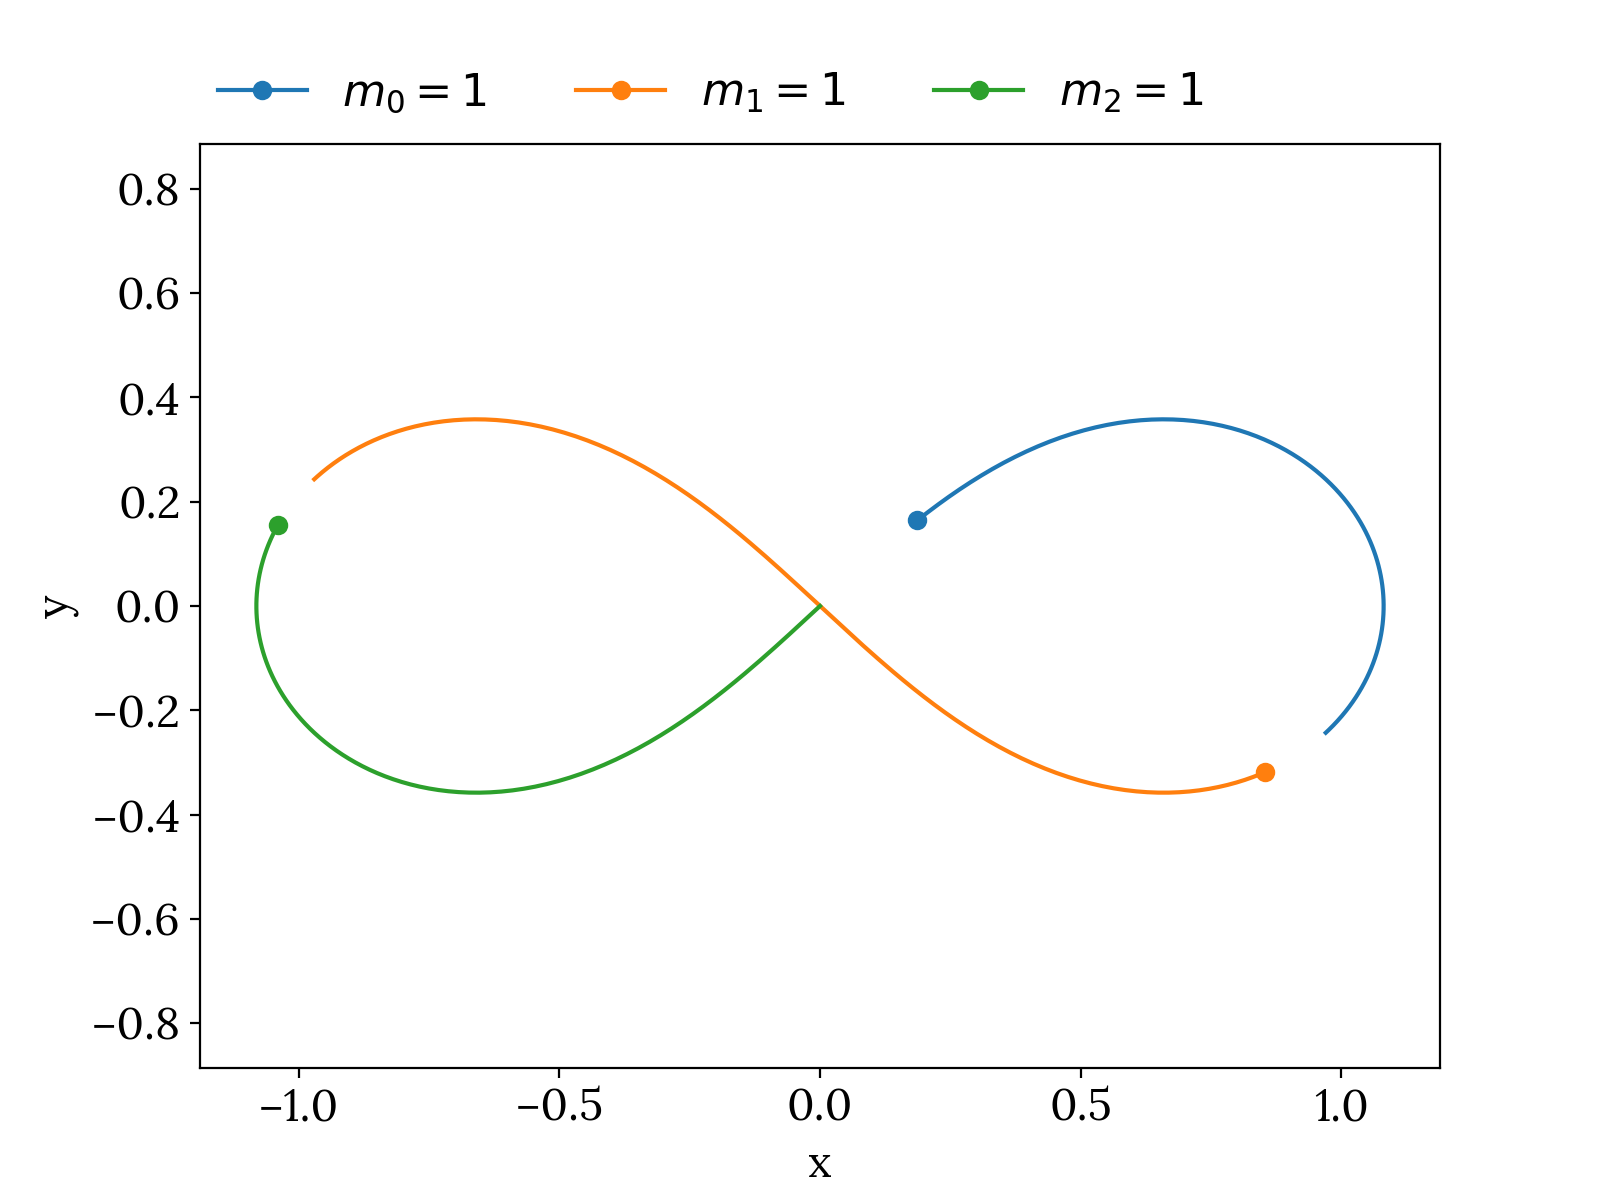
\includegraphics[width=0.8\linewidth]{figure8.png}
 \caption{Trajectories of the three bodies of identical mass part way through the orbit. The trajectories appear to follow the Lemniscate of Bernoulli closely, a analytic figure of eight equation. }
 \label{fig:figure8}
\end{figure}

The program produces trajectories as shown in \cref{fig:figure8}. This following a figure of eight shape as expected. The energies and angular momenta are conserved similarly to \cref{ssec:twobody}. The angular momenta of the system at the start is zero and this is steady throughout as it only fluctuates on the order of $10^{-7}\%$. This test goes further to show the model solves problems of three bodies correctly as it matches the predicted paths shown from reference \cite{chenciner_remarkable_2000}.

\subsection{The Solar System}
This test models the planets of the Solar System to show the system works for astronomical units and bodies with different masses. The initial values were adapted from value from NASA data tables \cite{noauthor_planetary_nodate}. The initial conditions do not correctly encode the phase of the orbits and the orbits have been assumed to be circular. However, this is a good enough approximation for this test. These initial conditions are given in \texttt{bodies/solarsystem.json} \cite{dudgeon_oliverdudgeon/nbody_2019} and are in the astronomical units scheme from \cref{tab:unitsys}.The trajectories obtained from solving this system shown in \cref{fig:solarsystem}.

\begin{figure}[h]
 \centering
 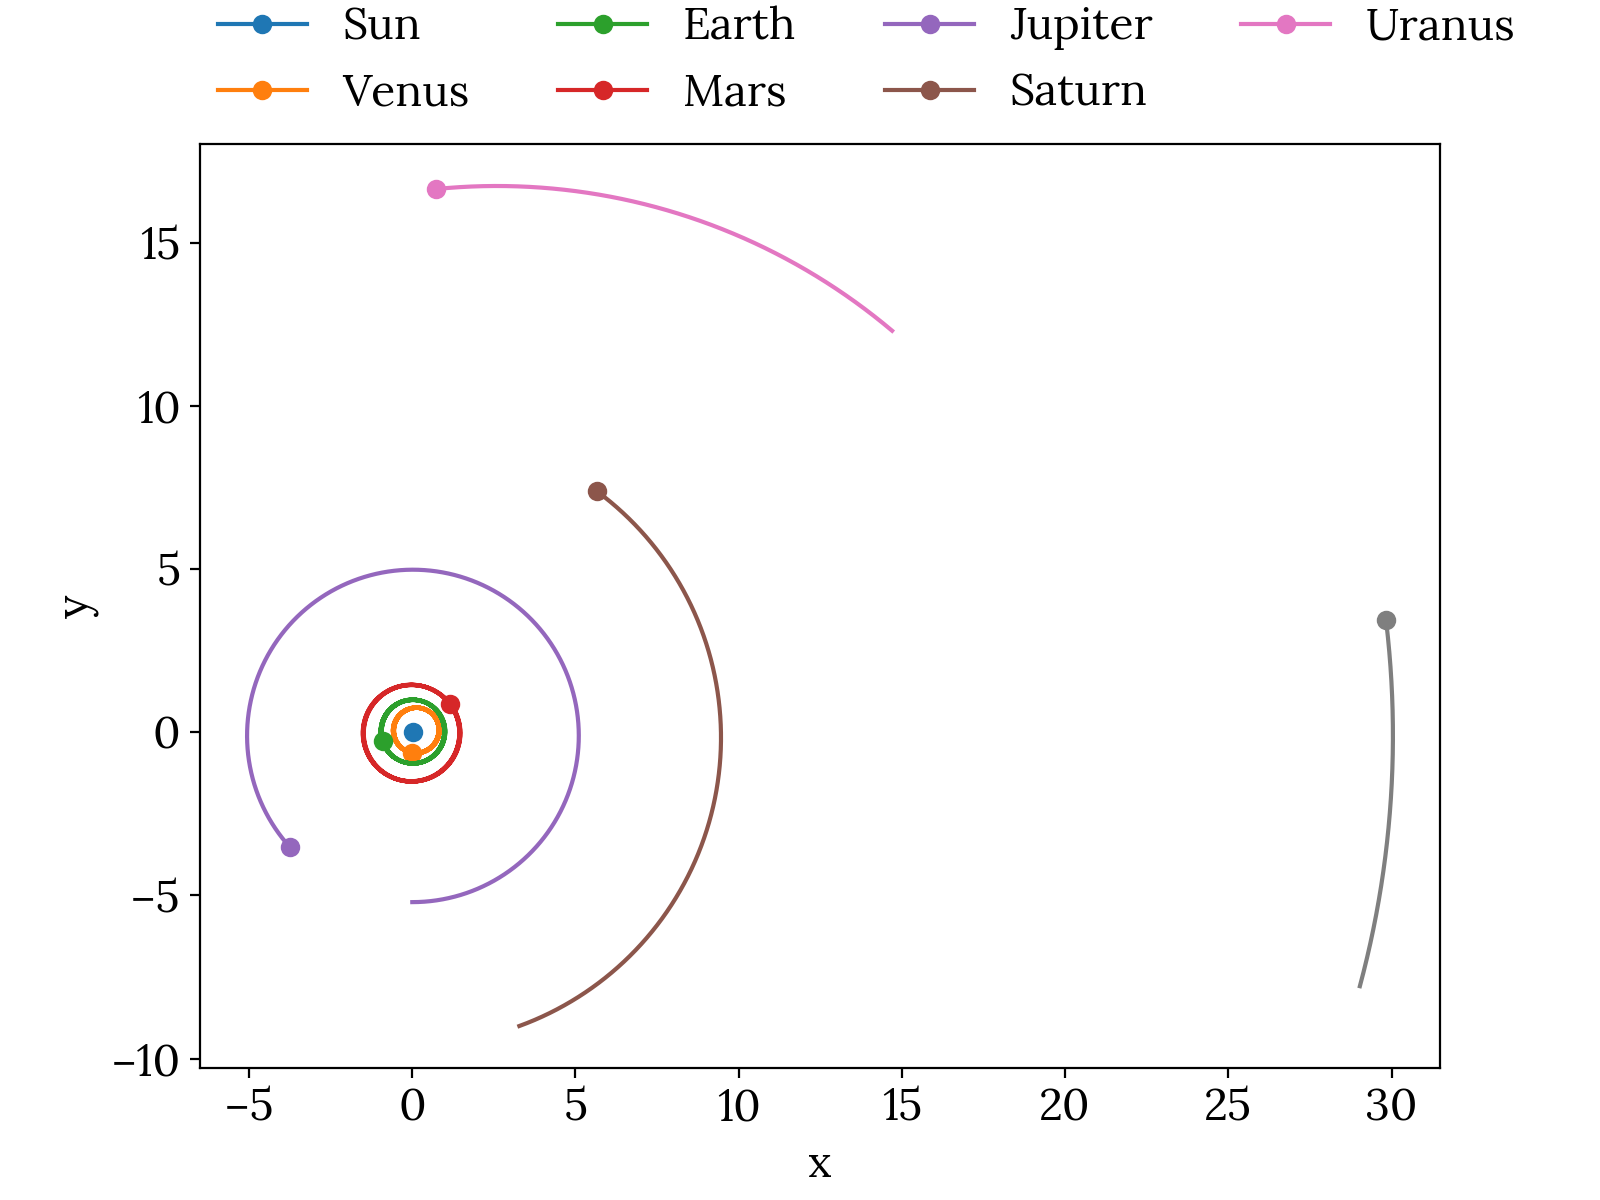
\includegraphics[width=1\linewidth]{solarsystem.png}
 \caption{Trajectories of the planets part way through the orbit. Mercury has been neglected as its orbit can only be explained when general relativity is taken into account. }
 \label{fig:solarsystem}
\end{figure}

The orbits are circular as expected which matches the observed orbits of the planets. The periods of the planets match up with the observed periods. Once again the relative change in energy is only on the order of $10^{-8}$. This does appear to increase steadily with time which is due to the accumulated numerical errors from the solver. However, for the short periods used this should not be a significant issue.

\section{Modelling Exoplanet Systems}

\subsection{Exoplanet Systems}

\begin{figure}[h]
 \centering
 \includegraphics[width=0.7\linewidth]{orbitalparams.pdf}
 \caption{Orbital parameters of importance in this report. $r$ is the distance from the origin to the point on the ellipse. $a$ is the semi-major axis of the ellipse --- half the length of the biggest axis of the ellipse. $i$ is the inclination angle, the angle between the orbital plane of the planet to the defined plane for the system. $v$ is the speed of the body which varies depending on the point in the orbit. Not shown here but also of importance is the eccentricity $e = \sqrt{a^2 - b^2} / a$, a measure of how elliptical the orbit is. $e = 0$ corresponds to circle and $0 < e < 1$ correspond to ellipses and are bound orbits. }
 \label{fig:orbitparams}
\end{figure}

Exoplanets are planets in the orbit around stars other than the Sun. Thousands of exoplanets have been confirmed thus far. These planets have been detected using numerous methods. A few examples include the transit method where a dip in the star's brightness is detected when a planet crosses between the star and the observer; direct imaging where the light reflected from the planet is detected and radial velocity, the method discussed later, where the doppler shifts in the star's brightness induced by planets is measured. Typically, the parameters measured are the mass, semi-major axis $a$, the eccentricity $e$, orbital period $P$ and the inclination $i$ not to be confused with the index label used so far. These values are summarised in \cref{fig:orbitparams} and are typically enough to model the system. The orbital speed of mass $m_i$, $i\neq 0$ when at a distance $r^{(i)} = |\vec{x}^{(i)}|$ can be determined using the vis-viva equation \cite{lissauer_fundamental_2014}:

\begin{equation}
 v^{(i)} = \sqrt{Gm_0\bigg(\frac{2}{r^{(i)}} - \frac{1}{a^{(i)}}\bigg)}
 \label{eq:visviva}
\end{equation}

where $m_0$ is the mass of the star. The distance value is set such that $r^{(i)} = a^{(i)}(1+e^{(i)})$. This is the greatest distance from the origin to the orbit. This allows the initial conditions to be set so that the magnitudes of the position and speed vectors are $r^{(i)}$ and $v^{(i)}$ respectively.

\subsection{Radial Velocity Detection}
As is evident from the two-body test example, \cref{fig:twobodies}, each body induces motion on the others. This means for planetary systems, the planets induce motion in the star. The star's emitted light has characteristic spectral lines at particular wavelengths. These are doppler shifted by the motion. By comparing the shifted wavelengths to values measured in the lab, the component of the velocity of the star in the direction from the star to the observer can be measured. This component is the radial velocity. Many very massive planets have been detected from analysis of radial velocity data. For this part of the project, data from the exoplanet archive \cite{noauthor_bulk_nodate} is used, where several radial velocity curves for various stars have been published.

The systems chosen to be investigated are detected using the radial velocity technique. The inclination values of the orbits are typically unknown, due to the limitations of the method, therefore the masses used are a minimum mass $M\sin i$. Furthermore, the orbits of the stars and planets are assumed to be coplanar.

\subsection{Fitting a Radial Velocity Curve}
Real-world data is now to be fitted using the model. The system HD 2039 is an exoplanetary system consisting of a yellow-dwarf star with a mass of $1.2\ \mathrm{M_\odot}$ and a single planet of around 6.11 Jupiter masses. The system is about 280 light-years away from Earth.

\begin{table}[H]
 \centering
 \caption{Parameters of the HD 142 system \cite{noauthor_open_nodate}. The values are given in astronomical units outlined in \cref{tab:unitsys}.}

 \setlength{\tabcolsep}{0.5em}
 \renewcommand{\arraystretch}{1.5}
 \begin{tabular}{|c|c|c|c|c|}
 \hline
 Body & $m$ & $a$ & $P$ & $e$ \\
 \hline
 Star & 0.980 & - & - & - \\
 \hline
 Planet b & $4.67\times10^{-3}$ & 2.20 & 3.24 & 0.670\\
 \hline
 \end{tabular}
 \label{tab:hd142}
\end{table}

The radial velocity curve has been measured by Butler et al. \cite{butler_catalog_2006} and Tinney et al. \cite{tinney_four_2003}. The data is available from the exoplanet archive. Using the model, the trajectories of the system are determined which are shown in \cref{fig:hd2039}. The relative change in energy and angular momentum are plotted in \cref{fig:hd2039stats}. The gradual variation in these conserved quantities occurs each period. This will only become significant after a large number of orbits.

\begin{figure}[H]
 \centering
 \includegraphics[width=0.6\linewidth]{hd2039.png}
 \caption{The trajectories of the HD 2039 system. The planet HD 2039 b orbits with the right period in an ellipse as expected.}
 \label{fig:hd2039}
\end{figure}

\begin{figure}[H]
 \centering
 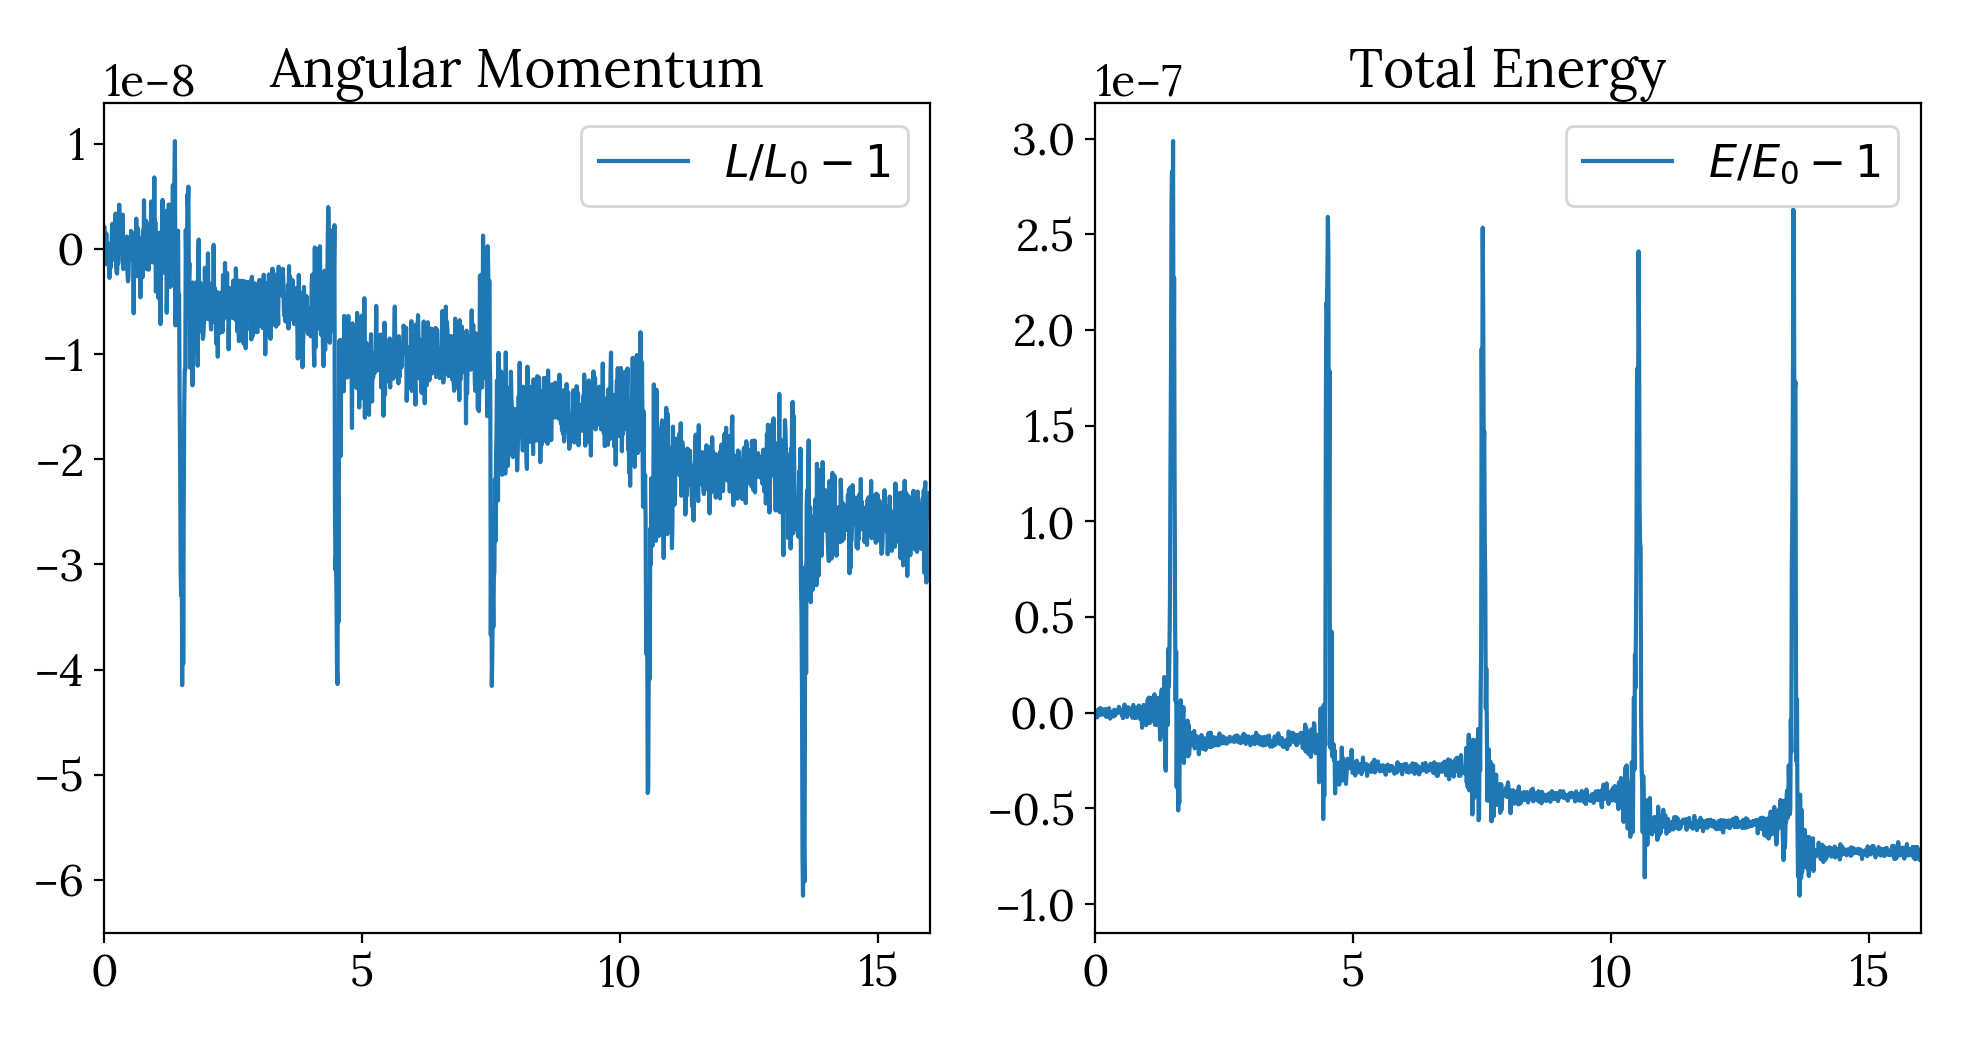
\includegraphics[width=\linewidth]{HD2039Stats.png}
 \caption{Relative change in energy and angular momentum with time. Each orbit the energy and angular momentum diverge away from the initial value. This is a small amount: $5\times10^{-7}\%$ for the energy and $t\times10^{-8}$ for the angular momentum. }
 \label{fig:hd2039stats}
\end{figure}


If the observer of such a system lies along the direction given by the unit vector $\hat{n}$ then the radial velocity detected by that observer is $v_r = \vec{v} \cdot \hat{n}$. In \cref{fig:hd2039dat100}, \cref{fig:hd2039dat010} and \cref{fig:hd2039dat110} three extremes of the possible directions are illustrated. These are all edge-on views, that is the unit vector $\hat{n}$ is completely in the orbital plane.

\begin{figure}[H]
 \centering
 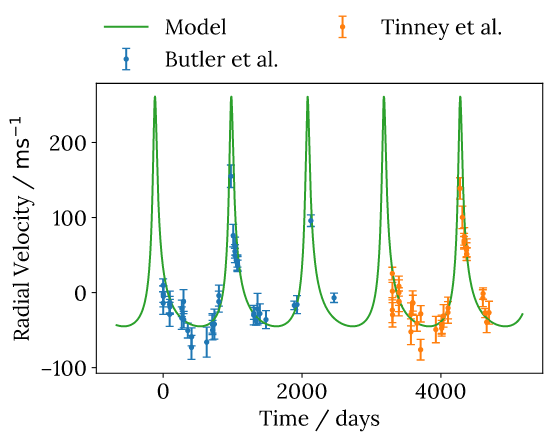
\includegraphics[width=0.6\linewidth]{hd2039dat010.png}
 \caption{The radial velocity curve from the model for the unit vector $\hat{n} = (0, 1, 0)$, fitting the empirical data points. The phase of the two sets has been adjusted to fit the model. This does not however change the magnitude of the radial velocity. }
 \label{fig:hd2039dat010}
\end{figure}

\begin{figure}[H]
 \centering
 \begin{minipage}{0.45\textwidth}
 \centering
 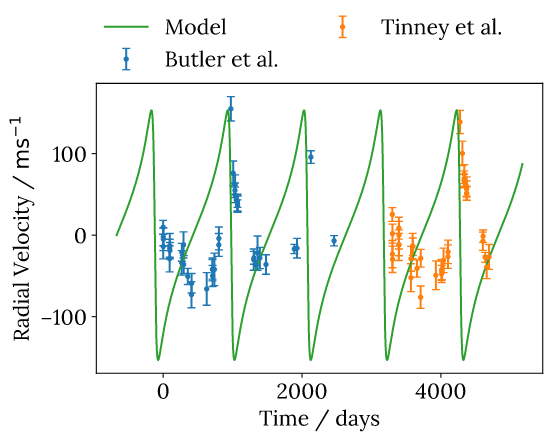
\includegraphics[width=\linewidth]{hd2039dat100.png}
 \caption{The radial velocity curve and the data points for the unit vector $\hat{n} = (1, 0, 0)$. The points do not fit the curve well at all. This is the wrong direction for $\hat{n}$. }
 \label{fig:hd2039dat100}
 \end{minipage}
 \hfill
 \begin{minipage}{0.45\textwidth}
 \centering
 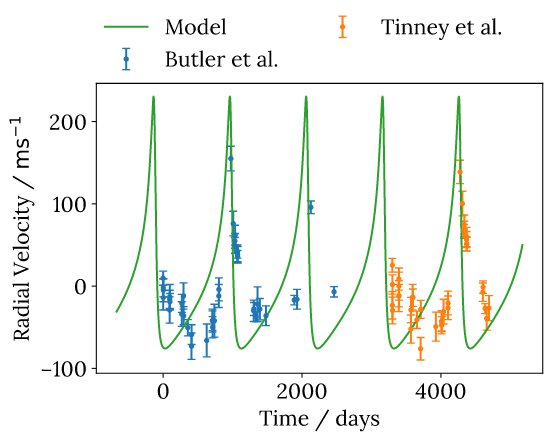
\includegraphics[width=\linewidth]{hd2039dat110.png}
 \caption{The radial velocity curve and the data points for the unit vector $\hat{n} = (1/\sqrt{2}, 1/\sqrt{2}, 0)$. The curve fits better than \cref{fig:hd2039dat100} but not as well as \cref{fig:hd2039dat010}. This is also not the right direction for the radial velocity. }
 \label{fig:hd2039dat110}
 \end{minipage}
\end{figure}

The curve from \cref{fig:hd2039dat010} fits the data best so the determined values for the parameters of the system \cite{noauthor_open_nodate-1} are consistent with the model shown here along with an observation direction that is edge-on.

More complex planetary systems theoretically could be fitted with this model. However, the large number of degrees of freedom in such systems makes it difficult to find the right parameters. Using linear regression (fitting a model to data) could achieve this but it is possible such a program would converge on solutions that match the data well but not the actual system. Concretely, several systems can be consistent with a particular radial velocity data set. The system could converge on the incorrect value.

\section{Summary}

The N-body problem is a class of physical systems where several masses interact gravitationally and the future trajectories of the system are wanted given the parameters at a given time. In this project, a python program to solve N-Body systems in two and three dimensions has been developed. This uses the Runge-Kutta algorithm of fourth-order. Astronomical units were used to encode the initial conditions stored in JSON files. Once loaded the system is solved and the trajectories are cached for future use.

The program solves most orbits (those without close encounters) well with only a small deviation in the total energy and total angular momentum. Therefore, this solver should not be used on systems with close encounters or when a large number of orbits are desired as such trajectories may become unphysical. The model does not take into account collisions between bodies. Better algorithms exist to solve this problem and conserve energy and angular momentum batter than Runge-Kutta however it was suitable for the systems investigated.

The solver was tested on a variety of systems. Two-body systems produced the expected elliptical orbits and it was found to match the figure of eight systems well. The Solar System was modelled to have accurate periods except for Mercury which could not be explained using Newtonian physics.

The model was used to investigate whether empirical radial velocity data could be fitted to a radial velocity curve produced from the motion of the stars from the model. It was found to be possible for simple systems where a single planet was involved but it could not be achieved for more complex systems. An improved version of this system could use linear regression and machine learning to fit the free parameters to the empirical data. The parameters of the bodies and the direction to take the radial velocity from would be varied until a best-fit for the data was found. This would require far more development time. This issue means the model is unfortunately not suitable for this application.

\newpage
\printbibliography

2992 Words (excluding figure captions and references)

\end{document}
